\begin{figure}[!ht]
	\begin{subfigure}[t]{0.5\textwidth}
		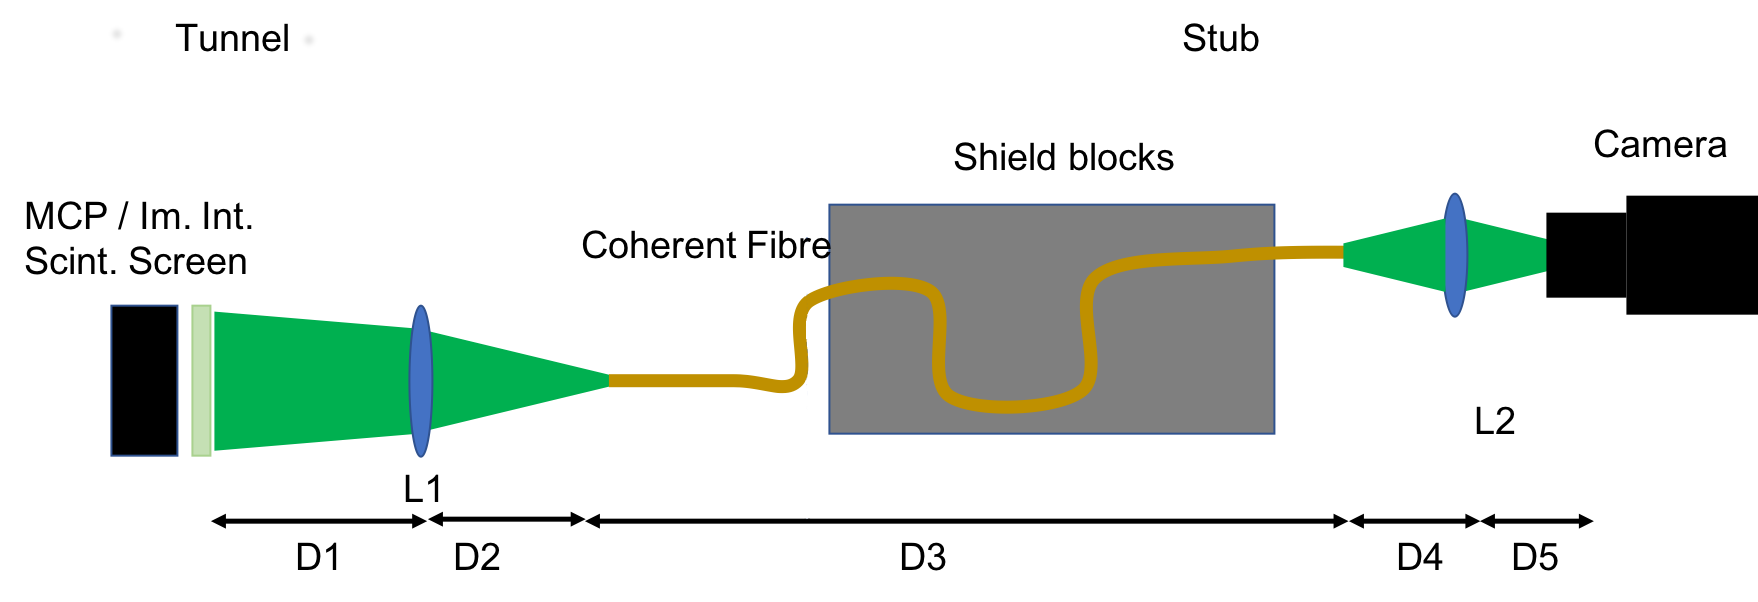
\includegraphics[width=\textwidth]{05_Conclusion/figures/fig000_schematic_coherentr_fiber}
		\caption{The profile image is transported through an optical fiber bundle.}
		\label{chap5:fig:schematic:1}
	\end{subfigure}
	~
	\begin{subfigure}[t]{0.5\textwidth}
    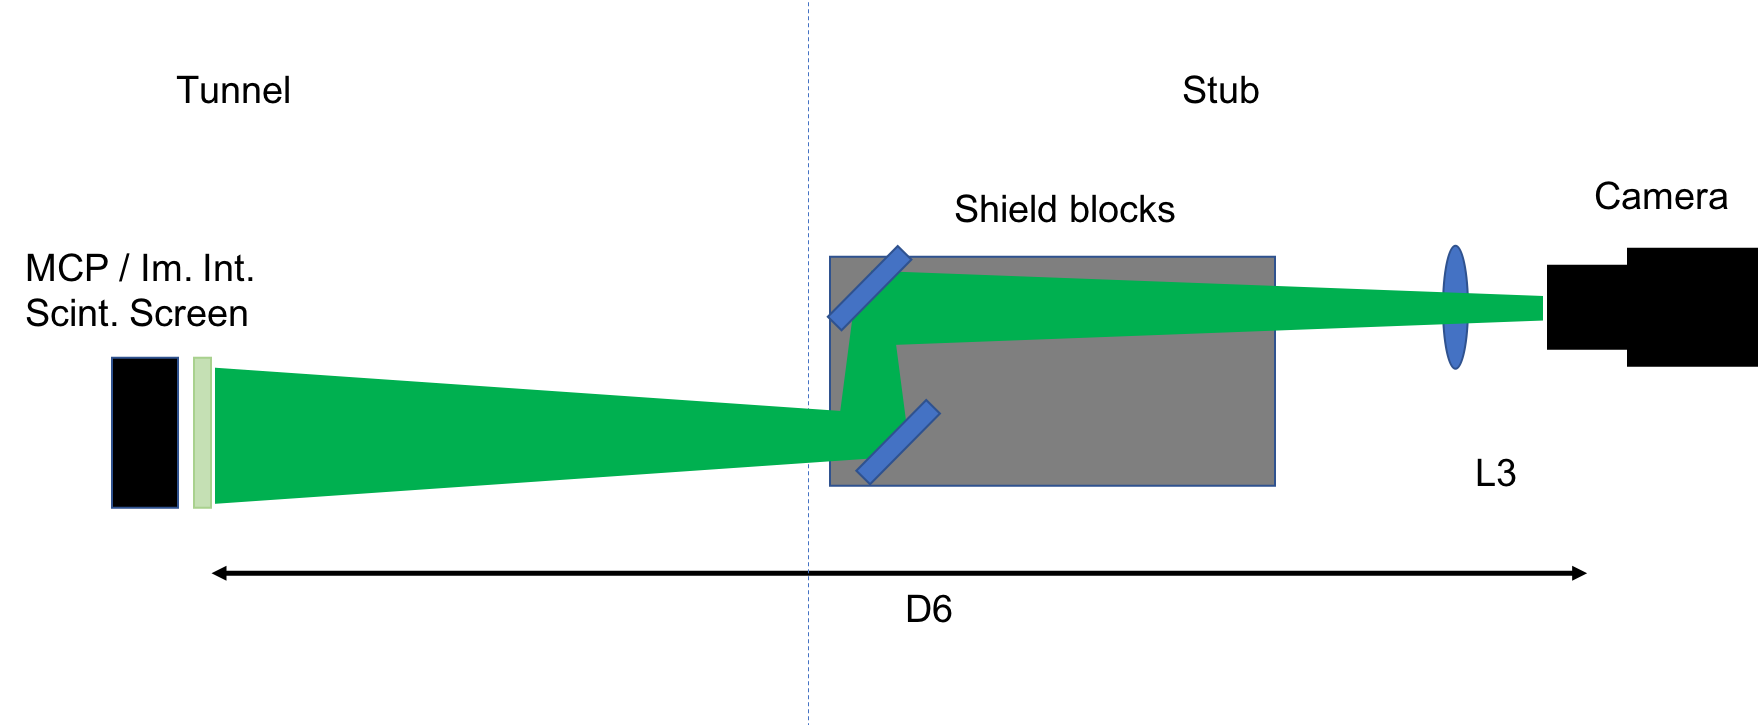
\includegraphics[width=\textwidth]{05_Conclusion/figures/fig000_schematic_telescop_lens}
		\caption{The profile image is reflected on mirrors.}
		\label{chap5:fig:schematic:2}
	\end{subfigure}
	\caption[Two solutions are forseen for remote acquisitions of the profile measurement]{Two solutions are forseen for remote acquisitions of the profile measurement \cite{CyrilleCDR2019}.}
	\label{chap5:fig:schematic}
\end{figure}
